% \documentclass{article}
% \usepackage[utf8]{inputenc}
% \title{Mathematical analysis of CAD Software}
% \author{Ankush Shaw and Anirudh Khammampati}

% \begin{document}
% \maketitle%(Type your content here.)
% \end{document}
\documentclass{article}
\usepackage{geometry}
\usepackage{graphicx}
\usepackage{bm}
\usepackage{amsmath}
\usepackage[utf8]{inputenc}
\usepackage{titling}
\usepackage{amsfonts}
\usepackage{titlesec}
\usepackage{amsmath}
\DeclareMathOperator{\taninv}{tan\,inverse}
\geometry{
a4paper, 
top = 1.5in
}
\graphicspath{ {Images/} }
\titlespacing*{\section}
{0pt}{6.5ex plus 1ex minus .2ex}{2.3ex plus .2ex}
\setlength{\droptitle}{10em}
\title{\huge{\textbf{Mathematical Analysis of CAD Software}}}
\author{\large{Ankush shaw \, Anirudh Khammampati}}
\date{\large{Indian Institute of Technology, Delhi}}

\begin{document}

\maketitle
\newpage
\tableofcontents
\newpage

\section{Abstract}
\indent The Computer Aided Software (long for CAD) is one of the many and a major area in which computers can be used to enhance the engineering that goes behind the greatest things we witness around. This is yet another try on developing a CAD software themed on simplicity in terms of use. This is a part of the Design Practices course here at IIT, Delhi. \par
This document states the assumptions, simplification, discusses the ideas and explain the mathematics behind it.
\section{Overview of Design}
Before delving into the mathematics aspects of the project we would have to decide a couple of things. We have to ascertain them as mathematics for the software package would change accordingly. We use the celebrated  polygon mesh technique to store the object. This is discussed briefly in \textbf{section 3.1}. Having decided on that we have to look for the ways in which user would input its object. We would provide support for both options, either interactively draw the object just like in generic CAD tools or input the object file in the prescribed format \textbf{section 3.2}. User can use features such as lines, rectangle, polygon (generalization), extrude \textbf{section 6.1}, cut \textbf{section 6.2} while in interactive mode. These tools makes the exhaustive set required to draw any polyhedral 3D object which one can think of. User has the luxury to rotate the object on the screen by the drag of the mouse and inspect it. At the top right corner we have a simple and narrative enough way to convey the current view with respect to object/coordinate system. \textbf{section 5} discusses the mathematics required for isometric or 3D to orthographic projection. User can obtain the isometric top, front, back, left \& right view of its 3D object.In this section we will also discuss about the mathematics  required for displaying a 3D object on a 2D screen which would continue into \textbf{section 6.4}. User also have a feature to find the distance between the required points on screen and he can even label and dimension them, something he has to do. \textbf{section 5} starts with the study of few 3D objects and provides enough examples as to why it is not deterministically possible to obtain the 3D model even with the 3 different orthographic views. Following which is the description of the assumptions about the permissible corresponding 3D objects and a discussion on the mathematics for the 2D views to 3D object derivation. Document ends at \textbf{section 6} which contains the mathematics for other features used/made available in the software package.

\section{Design choices}
\subsection{Data structure to store the object in memory}
We are storing the list of vertices, edges and faces for an object. The portion/volume being cut, if at all, from the otherwise perfectly convex objects would be stored separately in the form of vertices, edges and faces for further easy computation and rendering. For instance consider object given in the \textbf{figure 1.a}. this can be generated from the perfect convex object in the \textbf{figure 1.b} after removing the material equivalent to object in the \textbf{figure 1.c}.  
\begin {center}
	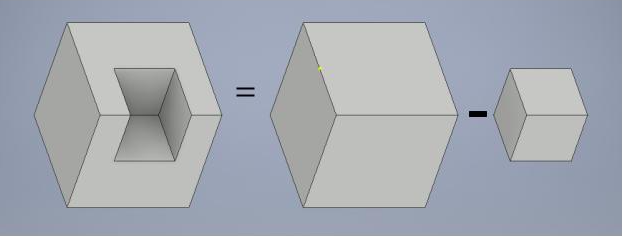
\includegraphics[height = 4cm]{fig1.png}\\
    \textbf{Fig 1.a,b,c}
\end {center}
\subsection{IO operations}
User of the software can either provide the data in the custom file format described in the \textbf{next subsection} or can draw it interactively in the \textbf{software's GUI}. Output would be displayed on the GUI of the software. User has the luxury to rotate and inspect the object in 360 degrees. They can change the view of the object with the help of the perspective cube at the top right corner of the GUI or with the mouse drag. They can zoom in and out with the scroll of the mouse. 

\subsection{File format}
File format chosen is custom in order to parse it easily yet making it easy for the layman to follow the format. User can use general statements like \textbf{A = (x, y, z)} to specify the location of the point and also make a reference of that point so that they wouldn't have to type the coordinates again while dictating the list of edges or faces.
In a file we would first have a list of vertices which also work as a reference to be used later,like above example followed by edge list and the face list in the end.
Each line should contain a single entity it can be either a vertex or a 2-tuple for an edge or a 3-tuple for a face. Further, if there is any cut/negative extrude in the object, user has to specify separately. He can append that information after the face list of the object in the similar convention used above starting with the keyword hidden in the line just followed by the last face element of the object. For instance, suppose we want to give data corresponding to the object in the \textbf{figure 1.a} of side length 20 units with the origin on the vertex on left side,bottom face, away from the user. \\ \\
vertex\\
a = 0, 0, 0\\
b = 20, 0, 0\\
c = 20, 20, 0\\
d = 0, 20, 0\\
e = 0, 0, 20\\
f = 20, 0, 20\\
g = 20, 20, 20\\
h = 0, 20, 20\\
edges\\
a, b\\
b, c\\
c, d\\
d, a\\
e, f\\
f, g\\
g, h\\
h, e\\
a, e\\
b, f\\
c, g\\
d, h\\
faces\\
a, b, c, d\\
e, f, g, h\\
a, b, f, e\\
b, c, g, f\\
c, d, h, g\\
d, a, h, e\\
hidden\\
vertex\\
a1 = 0, 0, 10\\
b1 = 20, 0, 10\\
c1 = 20, 20, 10\\
d1 = 0, 20, 10\\
e1 = 0, 0, 20\\
f1 = 20, 0, 20\\
g1 = 20, 20, 20\\
h1 = 0, 20, 20\\
edges\\
a1, b1\\
b1, c1\\
c1, d1\\
d1, a1\\
e1, f1\\
f1, g1\\
g1, h1\\
h1, e1\\
a1, e1\\
b1, f1\\
c1, g1\\
d1, h1\\
faces\\
a1, b1, c1, d1\\
e1, f1, g1, h1\\
a1, b1, f1, e1\\
b1, c1, g1, f1\\
c1, d1, h1, g1\\
d1, a1, h1, e1\\
\\
\textbf{Note:} \\ \indent 1. Observe that user has to first input coordinates for \textbf{fig1.b} followed by the information for the cut portion, i.e., \textbf{fig1.c}.
\\ \indent 2. Permissible keywords are \textbf{vertex, edges, faces \& hidden} and all characters in the keywords are in small case. \\ \indent 3. Though user can use large case characters for the reference names. 
\\ \indent 4. There is no restriction on the use of white-space. User can can have any amount of whitespace or none at all on the either side of the "=" or ",". 
\\ \indent 5. Only one entry per line is allowed.
\\ 
\section{Definitions for this analysis}
This section describes the notation and definition which will be used from here onwards in this analysis.
\\
\indent 1.$\mathbb{V}$ will be used for the matrix which contains the column vectors of the distinct vertices of the object.\\
\indent 2.$\mathbb{V}'$ will be used for the matrix which contains the column vectors of the distinct vertices of the object formed by the hollow/cut portion, figure 1.c, of the otherwise convex object.
\\
\indent 3. \textbf{V, E, F, $V_H$, $E_H$ \& $F_H$} represents the set of vertices, edges and faces for object and cut/hollow portion respectively in order.
\\
\indent 4. $\hat{v}, \hat{e}$ represents the vector representation of a vertex and an edge respectively. And $\hat{n}$ represent the vector in the direction of the perpendicular to the the plane under consideration.

\section{Orthographic to Isometric and back}
\subsection{3D to 2D}
\subsubsection{3D to Orthographic Projections}
\indent In this section we are going to find all the orthographic projections of a 3D object.We will project a 3D object onto some arbitrary plane so that we can generalize it for any plane.\par
let the equation of arbitrary plane be \(ax+by+cz+d=0\) and hence one of the vector perpendicular to the plane will be $(\hat{a},\hat{b},\hat{c})$. Let the following matrix represents the vertices of a 3D object where \(i^{th}\) column \:\((x_i,y_i,z_i)\) corresponds to coordinates of the \(i^{th}\) vertex denoted by $v_i$ of the given object. Let this matrix be $\mathbb{V}$
 \[
 \mathbb{V} =  
 \begin{bmatrix}
    x_{1}       & x_{2} & x_{3} & \dots & x_{n} \\
    y_{1}       & y_{2} & x_{3} & \dots & y_{n} \\
    z_{1}       & z_{2} & z_{3} & \dots & z_{n}
\end{bmatrix}
\label{e1}\]\\
Parametric equation of line passing through the point P\((x_0,y_0,z_0)\) and with $ \vec{a}, \vec{b}, \vec{c}$ as its directional ratios will be of the form  \[ 
		\mathbb{L} :   \begin{bmatrix}
         x  \\
         y    \\
         z     
         \end{bmatrix} 
         =
         \begin{bmatrix}
         x_0   \\
         y_0    \\
         z_0     
         \end{bmatrix} + \lambda
         \begin{bmatrix}
         a  \\
         b    \\
         c     
         \end{bmatrix} 
         =
         \begin{bmatrix}
         x_0 + \lambda a\\
         y_0 + \lambda b \\
         z_0 + \lambda c 
         \end{bmatrix}
         \quad where \lambda \  \textrm{is a scalar} \]\\
	Similarly for matrix $ \mathbb{V} $ , i.e., distinct lines through $v_i$ along the direction $ \vec{a}, \vec{b}, \vec{c}$ \:
    $$ 
    \begin{bmatrix}
    a \\
    b \\
    c \\
    0 \\
    \end{bmatrix}
    \begin{bmatrix}
    \lambda_{1} & \lambda_{2} & \lambda_{3} & \dots  &\lambda_{n}
    \end{bmatrix}
    + 
    \begin{bmatrix}
    x_{1}       & x_{2} & x_{3} & \dots & x_{n} \\
    y_{1}       & y_{2} & x_{3} & \dots & y_{n} \\
    z_{1}       & z_{2} & z_{3} & \dots & z_{n} \\
    1 & 1 & 1& \dots & 1 
\end{bmatrix}
 = 
 \begin{bmatrix}
 a\lambda_{1} & a\lambda_{2} & a\lambda_{3} & \dots & a\lambda_{n} \\
 b\lambda_{1} & b\lambda_{2} & b\lambda_{3} & \dots &b\lambda_{n} \\
 c\lambda_{1} & c\lambda_{2} & c\lambda_{3} & \dots & d\lambda_{n} \\
1 & 1 & 1& \dots & 1 
 \end{bmatrix}
 $$
 And that is nothing but,
 $$
 \begin{bmatrix}
 x_1 + a\lambda_{1} & x_2 + a\lambda_{2} & x_3 + a\lambda_{3} & \dots& x_n + a\lambda_{n} \\
 y_1 + b\lambda_{1} & y_2 + b\lambda_{2} & y_3 + b\lambda_{3} & \dots& y_n + b\lambda_{n} \\
 z_1 + c\lambda_{1} & z_2 + c\lambda_{2} & z_3 + c\lambda_{3} & \dots& z_n + d\lambda_{n} \\
 1 & 1 & 1& \dots & 1 
 \end{bmatrix}
$$
For finding projection of an object we are going to project all vertex of the object to the projection plane and join all the edges between the vertices as defined by the \textbf{E} , edge set. We use  equation(2) for finding perpendicular projections from vertex to the plane.\\
Let the foot of perpendicular drawn from vertex \(V_i\) onto the plane \(ax+by+cz+d=0\) be \(x\prime ,y\prime ,z\prime \) and it should be in the form of \((x_i+\lambda_{i} a\,,y_i+\lambda_{i} b\,,z_i+\lambda_{i}c)\).
As this point lies in that plane hence it should satisfy its equation. And substituting this point in plane's equation we would get the value of  $\lambda_i$ and hence the corresponding foot.\[ \begin{bmatrix}
         a &  b & c & d
         \end{bmatrix} * \begin{bmatrix}
         x\prime   \\
         y\prime    \\
         z\prime    \\
         1
         \end{bmatrix} = 0\]\\
       Therefore, \\
      \[ \begin{bmatrix}
         a &  b & c & d
         \end{bmatrix} * \begin{bmatrix}
         x_i+\lambda_{i} a  \\
         y_i+\lambda_{i} b   \\
         z_i+\lambda_{i} c  \\
         1
         \end{bmatrix} = 0\]
      \[ \begin{bmatrix}
         ax_i+\lambda_{i}a^{2} + by_i+\lambda_{i}b^{2} + cz_i+\lambda_{i}c^{2}+d
         \end{bmatrix} = 0 \]
  \begin{gather}   
  \lambda_{i} = \frac{-(ax_i+by_i+cz_i+d)}{a^{2}+b^{2}+c^{2}} \\
   \end{gather}
Point of projection for vertex $V_i$ is
 
 $$ \begin{bmatrix}
         x_i+\lambda_{i} a  \\
         y_i+\lambda_{i} b   \\
         z_i+\lambda_{i} c 
  \end{bmatrix} $$ with corresponding $\lambda_{i}$ values. \\
After finding the projection of all the vertices on a plane we would connect all the corresponding vertices using the \textbf{E} set tuples.\\
Since we generated projection of a 3D object onto a arbitary 2D plane now we can find its projections onto any specific plane , i.e., xy, yz, zx plane by substituting its plane equation.\\
Suppose we consider viewing along z-axis as \textbf{top-view} view then that is equivalent to the projection on a plane parallel to xy-plane.
Finding projection of given object onto xy-plane:
Equation of xy-plane is \(z=d\) \qquad $\Rightarrow$ \(a=0\,,b=0\,,c=1\,,d=d\)\\
 So, the value of $\lambda_{i}$ corresponding to  vertex $V_{i} $
     \begin{gather}   
  \lambda_{i} = \frac{-z_i - d}{1}\\
   \end{gather}
 point of projection for vertex $V_{i}$ is 
   $$ \begin{bmatrix}
         x_i+\frac{-z_i -d}{1}*0  \\
         y_i+\frac{-z_i -d}{1}*0   \\
         z_i + \frac{-z_i - d}{1} * 1 
  \end{bmatrix} = \begin{bmatrix}
         x_i \\
         y_i \\
         d
  \end{bmatrix} $$
 $\Rightarrow$  projecting a 3d object onto \textbf{ plane parallel to xy-plane} changes the vertex matrix 
  from V to $V\prime $ by changing  the \textbf{z-coordinate} to the same value dependent on equation of  the plane\[
 \begin{bmatrix}
    x_{1}       & x_{2} & x_{3} & \dots & x_{n} \\
    y_{1}       & y_{2} & x_{3} & \dots & y_{n} \\
    z_{1}       & z_{2} & z_{3} & \dots & z_{n}
\end{bmatrix}
  -> \begin{bmatrix}
    x_{1}       & x_{2} & x_{3} & \dots & x_{n} \\
    y_{1}       & y_{2} & x_{3} & \dots & y_{n} \\
    d & d & d  & \dots & d
    \end{bmatrix}\]\\
    Eliminate the z coordinates 
    $$ 
    \begin{bmatrix}
    x_{1}       & x_{2} & x_{3} & \dots & x_{n} \\
    y_{1}       & y_{2} & x_{3} & \dots & y_{n} \\
    z_{1}       & z_{2} & z_{3} & \dots & z_{n}
\end{bmatrix}
  -> \begin{bmatrix}
    x_{1}       & x_{2} & x_{3} & \dots & x_{n} \\
    y_{1}       & y_{2} & x_{3} & \dots & y_{n}
    \end{bmatrix}
    $$
Similarly, for the front and side views we project the object onto \textbf{xz-plane} and \textbf{yz-plane} respectively.Also the vertex matrix changes accordingly by eliminating \textbf{y-coordinate} and \textbf{x-coordinate}.\\
\subsubsection{3D to Isometric projections}
An isometric view for an object can be obtained by choosing the viewing direction such that the angles between the projections of the x, y, and z axes are all the same, or 30$^\circ$.We can also interpret as viewing along one of the corner of a cube. So, the plane on which the Object is going to be projected should have its normal direction along cube diagonal.\par
There are eight different orientations to obtain an isometric view depending into which octant we are looking at. For simplicity lets consider projecting an object when viewing in first octant and to solve this we are rotating the object around y-axis here by the diagonal lets say $\beta$ ( here $\beta=45\deg $) and then  rotation of object around horizontal by $\alpha$ diagonal makes an angle $\alpha=\arcsin\frac{1}{\sqrt{3}}$.\\
let $V_o$ be the vertex matrix of the given 3d object and $R_1$ and $R_2$ are the rotation matrices along vertical and along horizontal direction and $V_{iso}$ is the obtained coordinates for the isometric view in first octent.
\[
 \mathbb{R_1} =  
 \begin{bmatrix}
    1      & 0 & 0  \\
   0      &\cos\alpha & \sin\alpha   \\
    0      &-\sin\alpha & \cos\alpha  
\end{bmatrix}\] 
\[
 \mathbb{R_2} =  
 \begin{bmatrix}
    \cos\beta      & 0 & -\sin\beta  \\
    0     & 1 & 0   \\
    \sin\beta      &0 & \cos\beta 
\end{bmatrix} \]
\[\mathbb{V_o} =  
 \begin{bmatrix}
    x_{1}       & x_{2} & x_{3}  & \dots & x_{n} \\
    y_{1}       & y_{2} & x_{3}  & \dots & y_{n} \\
    z_{1}       & z_{2} & z_{3}  & \dots & z_{n}
\end{bmatrix}\]
\[
 \mathbb{V_iso} =  
 \begin{bmatrix}
    x_{1}\prime       & x_{2}\prime & x_{3}\prime & \dots & x_{n}\prime \\
    y_{1} \prime      & y_{2}\prime & x_{3}\prime  & \dots & y_{n}\prime \\
    z_{1}\prime       & z_{2}\prime & z_{3}\prime   & \dots & z_{n}\prime
\end{bmatrix}\]
$$
 \begin{bmatrix}
    x_{1}\prime       & x_{2}\prime & x_{3}\prime  & \dots& x_{n}\prime \\
    y_{1} \prime      & y_{2}\prime & x_{3}\prime  & \dots & y_{n}\prime \\
    z_{1}\prime       & z_{2}\prime & z_{3}\prime  & \dots & z_{n}\prime
\end{bmatrix} =
 \begin{bmatrix}
    1      & 0 & 0  \\
   0      & \cos\alpha & \sin\alpha   \\
    0      & -\sin\alpha & \cos\alpha  
\end{bmatrix} *
 \begin{bmatrix}
    \cos\beta      & 0 & -\sin\beta  \\
    0      &1 & 0   \\
    \sin\beta      &0 & \cos\beta 
\end{bmatrix} *
 \begin{bmatrix}
    x_{1}       & x_{2} & x_{3}  & \dots& x_{n} \\
    y_{1}       & y_{2} & x_{3}  & \dots & y_{n} \\
    z_{1}       & z_{2} & z_{3}  & \dots & z_{n}
\end{bmatrix} 
$$


 Now we need to project it on to \textbf{xy-plane} so to obtain isometric projection in first octant.let the the vertex matrix obtained after projecting on to xy plane be $V\prime_{iso}$\\
 \[\mathbb{V\prime_{iso}} =  
 \begin{bmatrix}
    1      & 0 & 0  \\
   0      & 1 & 0  \\
    0      & 0 & 0 
\end{bmatrix} *
 \begin{bmatrix}
    x_{1}\prime       & x_{2}\prime & x_{3}\prime  & \dots& x_{n}\prime \\
    y_{1} \prime      & y_{2}\prime & x_{3}\prime  & \dots & y_{n}\prime \\
    z_{1}\prime       & z_{2}\prime & z_{3}\prime  & \dots & z_{n}\prime
\end{bmatrix} =
\begin{bmatrix}
    x_{1}\prime       & x_{2}\prime & x_{3}\prime & \dots & x_{n}\prime \\
    y_{1}\prime       & y_{2}\prime & x_{3}\prime & \dots & y_{n}\prime\
    \end{bmatrix}
\].\par
\indent Thus we obtained isometric projection of an 3D object when viewing from first octent .Similarly,we can compute  the isometric projection for any  3D object onto required plane by making Successive rotations and then projecting it onto the plane. 
 


\subsubsection{Hidden edges}
In this subsection we will discuss how to handle hidden edges in the orthographic projection. For this section take the conventional orientation of the axes as shown in \textbf{figure 2.a }. We will analyze the case of hidden lines in the front view.  Though similar analysis follows for top and side views.\\
\textbf{Fact:} Imagine all edges to be luminous. Only way we can't see a edge in the front view is when light emitted from the edge is not able to reach our eyes.\\
\indent Or we can say, that particular edge is occluded. When the eye is at infinity rays reaching the eye is that along the z axis. Equation of the plane formed by such rays is given by \textbf{equation 6 } below. Next step would be to consider all the planes formed by the faces of the object and check one by one whether these two intersect in a line or not. One caveat to be pointed out at this stage is that the solution obtained would be for the extended planes whereas what we want is intersection of the face of the object with the segment of plane formed by the edge along the z axis. We solve that in the following steps.\\
Let the end points of the edge which we want to analyse whether it is occluded by a face  be $\vec{p_1} \& \vec{p_2}$ then the vector along the edge is given by $\vec{p_2} - \vec{p_1}$, lets call that $\vec{e}$. And to find the equation of the plane containing the edge and along the z axis, we require a vector in the direction perpendicular to the plane and a point in the plane. One of the vectors perpendicular to the plane is:
$$ \vec{n} = \hat{j} \times \vec{e} $$ 
So the equation of the plane is
\begin {align} \vec{n} (\vec{x} - \vec{p}_1) = 0 \\
\vec{x}\dot\vec{n} = \vec{n}\dot\vec{p}_1
\end{align}
And the equation of the plane containing a face with the edges say $\vec{e}_1 , \vec{e}_2, \vec{e}_3, \vec{e}_4$ is given by
\begin{align}
	\vec{n}_1 = \vec{e}_1 - \vec{e}_2 \\
    \vec{x} . \vec{n}_1 = \vec{x}_\alpha . \vec{n}_1   
 \end{align}
 where $\vec{n} \ \& \  \vec{n}_1$ are the vectors perpendicular to the corresponding plane. And $\vec{x}_\alpha$ is the end point of any of the four edges which are contained in the plane (as assumed above).\\
 To find the line of intersection after checking if the planes are parallel or not, first find the direction ratio along that solution line that would be nothing but, 
 $$ 
 		\vec{r} = \vec{n} \times \vec{n}_1
$$
Let's call it $\vec{r}$ \\
Now all we need to find is the equation of that line is  a point lying on that line. We can find that by solving equation 6 \& equation 8 together with setting one of $\vec{x}, \vec{y} \ or\ \vec{z}$ component to be zero as we have more equations than independent variables. Lets call it $\vec{a}$. Then the solution would be of the form

\begin{align}
L = \vec{a} + \lambda\vec{r}
\end{align}
where $\lambda $ is a scalar (parameter).
\\
Coming to the caveat mentioned earlier that it might be the case that the line of intersection  actually lie out of the face completely. To solve this we would try to solve \textbf{equation 9} with the line equations of the four edges given below one by one which we initially thought to lie in the face we are currently analyzing. 
\begin {align}
L_1 : \vec{e}_{11} + \lambda \vec{e1} \\
L_2 : \vec{e}_{21} + \lambda \vec{e2} \\
L_3 : \vec{e}_{31} + \lambda \vec{e3} \\
L_4 : \vec{e}_{41} + \lambda \vec{e4} 
\end {align}
Where $\vec{e}_{i1} $ is either of the end points of $\vec{ei}$. Solve equation 8 (solution line) with all of then and note down the point of intersection. Let's call the intersection between equation 9 and $L_i$ 
\: $Intersection _i$.
\\
Then as $Intersection_i$ lies on the line $L_i$ therefore, it should also satisfy its equation. Obtain the corresponding $\lambda$ by solving the equation below. 
\begin{align}
Intersection_1 = \vec{e}_{is} + \lambda \vec{e(i)}
\end{align}\\
\textbf{Theorem:} If the value of the $\lambda$ is greater than 1 or less than 0 for all the distinct edges of the face then the edge is not occluded by the face under consideration. 
\\
\textbf{Proof:} (Intuition based) Let the end points of edge $\vec{ei}$ be $\vec{e}_{11} \ : \ C \ \&   \ \vec{e}_{12} \ : \ A $ (refer figure below). Then the equation of the Line $L_i$ becomes 
\begin{align}
L_i : \vec{e}_{i1} + \lambda \vec{e}_{2i} - \vec{e}_{1i}
\end{align}
\begin{center}
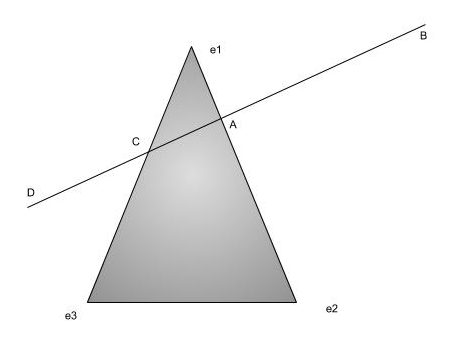
\includegraphics[height = 3cm]{figx.png}
\end{center}

When $\lambda = 1$, that corresponds to $\vec{e}_{2i}$. And when $\lambda = 0$, we get $\vec{e}_{1i}$. As we increase $\lambda$ we get points on AB ray. And for the values of $\lambda $ less than 0 we get points on the ray CD. \\
So for the point of intersection to be on the edge $\lambda$ has to be between 0 and 1.\\
Now, if $\lambda$(s) for all the four intersection is not between 0 and 1 then we can infer that line of intersection of planes (equation 9) does not cross through any of the edges of the face contained in the plane we are analyzing. Hence it won't cut the face and so won't be occluded by this face. 

\subsection{2D to 3D}
\subsubsection{Assumptions}
We make following assumption to solve this part:

\indent \textbf{1.} We assume that the volume of the closed object formed by any set of adjacent faces is non-zero. Because if not, even with 3 orthographic 2D views we would not be able to uniquely develop the corresponding 3D object. Counterexample being
\begin{center}
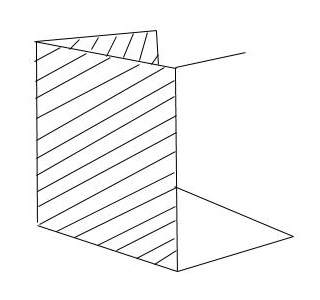
\includegraphics[height = 3cm]{fiz1.png}
\end{center}
\indent \textbf{2.} The object that is to be formed from the given orthographic projections must be either completely convex polyhedral or a concave polyhedral with a convex polyhedral cavity in it, where object could have been otherwise convex polyhedral if the cavity was not there.  \\
\begin{center}
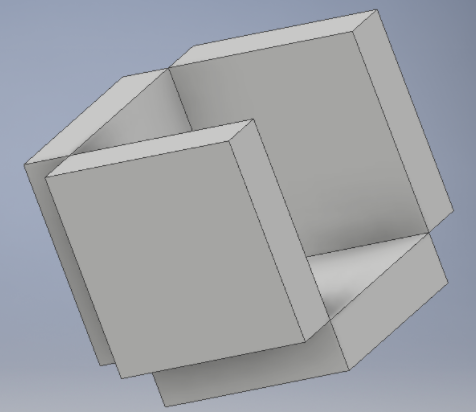
\includegraphics[height = 3cm]{figy.png}
\end{center}
\indent\textbf{3.}We want the user to specify all the hidden edges and occluded vertices separately because some hidden edges may coincide with other edges in the given orthographic projections. Without which it could not be possible to determine the 3D object accurately. Same goes for vertices too. \\
\indent \textbf{4.} For reducing the complexity while solving expressions we are considering \textbf{top view} corresponds to projection on \textbf{xy-plane} , \textbf{frontview} corresponds to the projection on \textbf{xz-plane} and the \textbf{sideview} corresponds to \textbf{yz-plane}. That is, we are assuming the coordinate system to be fixed with the object.\\
\subsubsection{Theorems}
1. \textbf{Two distinct orthographic projections are enough to uniquely locate a vertex in the 3D space.} \\
Every orthographic projection has one degree of information less ,i.e., they have lost information for one of the coordinates with the information intact for the other two. \\
We claim that no two distinct orthographic projection has information loss for the same axis. Because otherwise both projections would have information about the same two axes. But that contradicts the fact that those projections were distinct. Hence they have information loss about the different axis. \\
Hence, together they contains information for all the three axis.
Therefore with just two orthographic projections one can find out the $(x, y, z)$ for every point.\\
Let the matrix formed by vertices in top view be $\mathbb{V_t}$
, in front view be $\mathbb{V_f}$ and in side view be  $\mathbb{V_s}$
 where $i^{th}$ column in these three matrices is obtained by projecting vertex $V_i$ of object onto corresponding plane.
 \[
 \mathbb{V_t} =  
 \begin{bmatrix}
    x_{1}       & x_{2} & x_{3} & \dots & x_{n} \\
    y_{1}       & y_{2} & x_{3} & \dots & y_{n} 
\end{bmatrix} ,\:
\mathbb{V_f} =  
 \begin{bmatrix}
    x_{1}       & x_{2} & x_{3} & \dots & x_{n} \\
    z_{1}       & z_{2} & z_{3} & \dots & z_{n} 
\end{bmatrix} ,\:
\mathbb{V_s} =  
 \begin{bmatrix}
    y_{1}       & y_{2} & y_{3} & \dots & y_{n} \\
    z_{1}       & z_{2} & z_{3} & \dots & z_{n} 
\end{bmatrix}\]\\
From these matrices $\mathbb{V_t}$,$\mathbb{V_f}$,$\mathbb{V_s}$ we can construct a matrix $V_{obj}$ corresponding to vertices of object in 3d space and its given by
\[
 \mathbb{V_{obj}} =  
 \begin{bmatrix}
    x_{1}       & x_{2} & x_{3} & \dots & x_{n} \\
    y_{1}       & y_{2} & x_{3} & \dots & y_{n} \\
    z_{1}       & z_{2} & z_{3} & \dots & z_{n} 
\end{bmatrix} \]
\\
\textbf{Note:} For this to work out we have to take the coordinates to be as shown in the figure below for the consistency
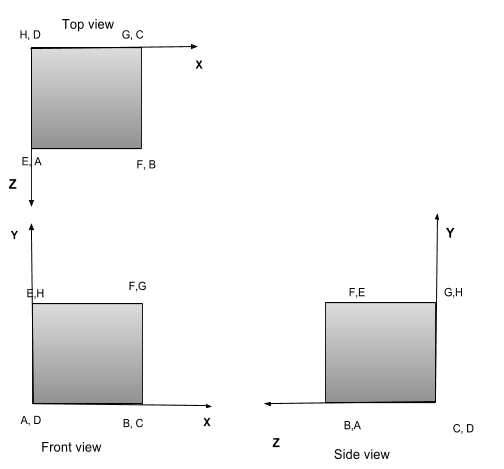
\includegraphics[height = 7cm]{gg.png}\\

2. \textbf{Following the  assumption that volume of the closed object  formed by the adjacent face subset is non zero and that permissible objects can only be convex polyhedral or concave polyhedral with convex polyhedral cavity refer fig1.a, every vertex is connected to atleast 3 other vertex}\\ 

\textbf{proof:} 
As the volume of the closed object formed by the group of adjacent faces is assumed to be non zero therefore at each vertex there should be an edge contributing to the non zero height, width and depth of the object to be. It might be the case where there are more a vertex is connected to more than 3 vertex as in the case of tip of pentagonal pyramid but it cannot be less than 3.\\
Proof by contradiction \: Assume the closed object formed the subset of \textbf{F} such that one of the vertex of a face is connected to only two other vertex. In such case, the object is not closed in the first place, which contradicts the assumption that the  object was closed. Because otherwise measure volume won't make sense for an object unless and untill it is closed. \\

\textbf{Transformation method adopted \:}\\
For explaining the method we will work along the object in \textbf{figure 1.a.}. Figure below shows the top, front \& side view for the object thought without the cavity and then the same procedure goes for the cavity having given some positive mass as a standalone object. In the end we subtract cavity's volume from the related convex polyhedral's volume. \\ 
\begin{center}
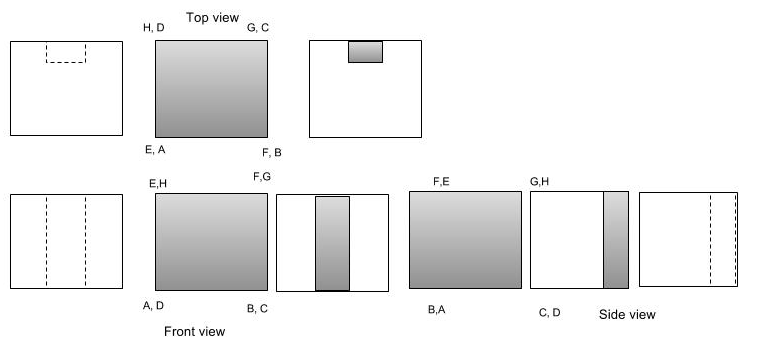
\includegraphics[height = 7cm]{aa.png}
\end{center}
Consider the point H in the top view. It could have been connected to D, G, C, A and E 
\begin{align}
\mathbb{H}_{top} = \{D, G, C, A, E\}
\end{align}
,i.e, it would be connected with the vertex on the other end of the edges connected to H or the vertex occluded by H directly.

Also, we can argue that H is connected to D , C and E out of the five possibilities mentioned about as the possibilities of edge for a vertex has to respect all the orthographic views in the sense that from front view the best of information we can extract for H is that it can be connected to,
\begin{align}
\mathbb{H}_{front} = \{E, A, D, F, G\}
\end{align}
Observe that connection to C is not a possibility for H from (17). Hence it is not connected to C as hinted by the top view. Similarly, we can argue that H is not connected to A accounting for the restrictions imposed by the side view. Therefore, out of the possibilities for H from the top view (equation 16) it could be connected with D, G and E. And as we know that a vertex has to be connected to at least 3 vertex hence it is exactly connected to D, G and E. Similar analysis follows for other vertics. \\
For the hidden part we can follow the similar approach. For instance, observe that the orthographic projection of the cut portion/volume accompanying the otherwise perfect convex polyhedral. From the three orthographic projection for the hidden volume. We can locate its vertices uniquely. And then argue the edge possibilities amongst them as illustrated in the paragraph above.\\
And while rendering the apparent 3D object will be obtained by making the hidden volume transparent. 

\textbf{Another approach: }Now, this above argument holds good for all the points. Therefore total number of maximum edges which can form is 
$$
	\textrm{max. possible edges} = \frac{\sum{\mathbb {E}_{i}}}{2}
$$
where $\mathbb {E}_{i}$ is the number of edges which have $i^{th}$ vertex at the either end. The maximum value of possible edges in this case would be $(8 * 3) / 2 = 12$. 

\section{Mathematics for miscellaneous features}
\subsection{Drawing tools}
For interactive input we would provide certain necessary drawing. These would be: \\
\\
\indent \textbf{1. Extrude }\\
To extend the selected face along a particular direction. \\
Let \textbf{x} be a vertex and \textbf{E} be the selected face. Also let $\alpha$ be the distance through which the face has been extruded then:\\
$$ \mathbb{V}' = \mathbb{V} \cup \{ \hat{x} + \alpha\hat{d} \ | \  x \in \textrm{E} \} \ ,where \ \hat{d} \ \textrm{is normal to E} $$
\\
\indent \textbf{2. Cut}\\
User can select a face, draw a 2D figure and cut through the object. All the information, i.e, vertex, edge \& face list for the volume which is being cut is stored separately in different lists for easy computation. Let $\zeta$ represent that 2D figure which would be used to cut and $\zeta_{V} \& \zeta_{E}$ be the set of vertices and edges formed then:
\begin{gather} 
V = \zeta_{V} \cup \{\hat{x} + \alpha \hat{d} \ | \ \forall \hat{x} \in \zeta_{V} \} \\
E = \zeta_{E} \cup \{(x, x + \alpha \hat{d} | \forall x \in \zeta_{V}  \} \cup \{(x_1 + \alpha \hat{d}, x_2 + \alpha \hat{d} | \forall x_1, x_2 \in \zeta_{v} \& x_1 \neq x_2 \} \\
F = \zeta \cup \{(x_1 + \alpha \hat{d}, x_2 + \alpha \hat{d} , x_3 + \alpha \hat{d}) \ | \ \forall x_1, x_2, x_3 \in \zeta_{v} \}
\end{gather}
Similarly, \textbf{V', E', F'} can be constructed in case of pyramidal cavity.\\
\subsection{Scaling}
\indent It is controlled by scrolling. For every unit of scroll object's size doubles. Where a 'unit' would depend on how platform returns the scroll information. For $\alpha$ units of scroll,

$$ \mathbb{V}' = \alpha \mathbb{V}, \quad \textrm{where} \ \alpha \ \textrm{is a scalar}$$
\subsection{Translation of object}
User can drag the object around the screen. After the translation \textbf{E \& F}, i.e., edge set and face set remains same whereas  $\mathbb{V}$ and hence \textbf{V} (vertices set) changes as follows
$$ \mathbb{V}' = 
 \begin{bmatrix}
    x_{1}       & x_{2} & x_{3} & \dots & x_{n} \\
    y_{1}       & y_{2} & x_{3} & \dots & y_{n} \\
    z_{1}       & z_{2} & z_{3} & \dots & z_{n}
\end{bmatrix}
+
\begin {bmatrix}
	x & \dots \\
    y & \dots \\
    z & \dots
   
  \end{bmatrix}
$$
Where (X, Y, Z) the vector through which the object has been dragged. \\
\textbf{Note:} Second matrix is added after proper broadcasting.

\subsection{Arbitrary projection on screen's plane for output display \& Output window Rotation}
After extracting the 3D object from the 2D projection we would still have to carry out further computation as we cannot show it as such to the user due to the limitation that screens we have are capable of 2D graphics only. More specifically we would have to take the projection of the object on the screen plane defined by the perspective cube at the top right of the GUI to be able to display it on the 2D screen.\\
Assume for this section that coordinate axis to be aligned with the screen, i.e, \textbf{X} and \textbf{Y} axes are along the width and height of the screen and \textbf{Z} axis is out of the screen towards the user. \\
Then dragging the cursor horizontally left would rotate the screen about the \textbf{Y} axis in the clockwise fashion. And dragging vertically down would rotate the object about the \textbf{X}.
To rotate about the \textbf{Z} axis use the perspective cube at the top right corner of the GUI.\\
For horizontal drag: rotates about Y axis. Hence Y coordinates remain unchanged where as X and Y coordinates goes under linear transformation as follows. 
$$
\mathbb{V}' = 
	\begin{bmatrix}
    \cos\theta &  0 & \sin\theta \\
    0 & 1 & 0 \\
    - \sin\theta & 0 & \cos\theta
    \end{bmatrix}
    \begin{bmatrix}
    x_{1}       & x_{2} & x_{3} & \dots & x_{n} \\
    y_{1}       & y_{2} & x_{3} & \dots & y_{n} \\
    z_{1}       & z_{2} & z_{3} & \dots & z_{n}
\end{bmatrix}
$$
Similarly, rotation about X and Z axis.\\
Using the method as described in the \textbf{sectino 5.1} take the front view projection and display on the screen without the hidden lines. We can further add texture and shadowing effect to make it look 3 dimensional.
Put images of cube being rotated along with the supplementary diagrams of the coordinate axis to help
\\
\\
\\
\\





\end{document}
